\documentclass{article}

\usepackage[letterpaper,top=2cm,bottom=2cm,left=3cm,right=3cm,marginparwidth=1.75cm]{geometry}
\usepackage{graphicx,subcaption,lipsum}
\graphicspath{ {./images/} }
\usepackage{float}
\usepackage[colorlinks=true, allcolors=blue]{hyperref}
\usepackage{listings}
\usepackage{color}
\usepackage{xparse}

\definecolor{dkgreen}{rgb}{0,0.6,0}
\definecolor{gray}{rgb}{0.5,0.5,0.5}
\definecolor{mauve}{rgb}{0.58,0,0.82}

\lstset{frame=tb,
	language=Bash,
	aboveskip=3mm,
	belowskip=3mm,
	showstringspaces=false,
	columns=flexible,
	basicstyle={\small\ttfamily},
	numbers=none,
	numberstyle=\tiny\color{gray},
	keywordstyle=\color{blue},
	commentstyle=\color{dkgreen},
	stringstyle=\color{mauve},
	breaklines=true,
	breakatwhitespace=true,
	tabsize=3
}

\title{
	Banco Multithread\\
	\large Relatório de implementação do trabalho 1\\INE5645 - Programação Paralela e Distribuída
}

\author{Giovane Pimentel de Sousa - 22202685\\
		Guilherme Henriques do Carmo - 22201630\\
		Isabela Vill de Aquino - 22201632
}
\begin{document}
\maketitle
\section*{Seção 1}
\section*{Introdução}
O trabalho solicitado consiste na implementação de um servidor multithreaded para realizar operações bancárias usando um pool de threads e o modelo de produtor/consumidor.

\section*{Decisões de Implementação}
A implementação foi realizada em \textbf{Golang} 1.23, utilizando apenas módulos da biblioteca padrão, em principal "\textit{sync}"
para toda a estrutura não sequencial, portanto, não é necessária a instalação de nenhum pacote adicional. Pensamos
em utilizar semáforos para controle de workers livres, porém em Go, a forma oficial é com channels, que implementa
dentro de si o controle de concorrência, o que era uma limitação estabelecida na definição do trabalho.

Foram esclhidas quatro parametrizações principais:
\textbf{número de threads trabalhadoras}, \textbf{número de clientes}, \textbf{número máximo de requisições}
que cada cliente efetuará e por fim o \textbf{tempo de serviço} (tempo de espera de cada operação).

Os clientes geram requisições em intervalos aleatórios e arbitrários de 0 a 5 segundos.

A variável \textit{numClients} foi definida para ser tanto relacionada à quantidade de clientes quanto de contas existentes no banco.

Foi escolhido pelo grupo um ponto de parada: \textbf{X} clientes atingirem \textbf{N} (maxRequests) requisições definida por parâmetro.
Portanto, quando o número de requisições atendidas pelos workers chegarem a X * N, o programa finaliza.

\section*{Como executar}
A sintaxe básica para execução é:
\begin{lstlisting}
	$ go run . [numWorkers] [numClients] [maxRequests] [serviceTimeInMiliseconds]
	# Então por exemplo:	
	$ go run . 1 3 1 1000
	$ go run . 2 5 2 300
\end{lstlisting}

Exemplos de execução:
\begin{figure}[H]
	\begin{subfigure}{.48\textwidth}
		\centering
		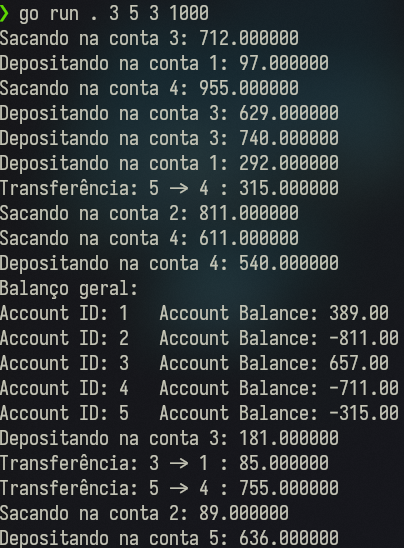
\includegraphics[scale=0.50]{1.png}
	\end{subfigure}
	\begin{subfigure}{.48\textwidth}
		\centering
		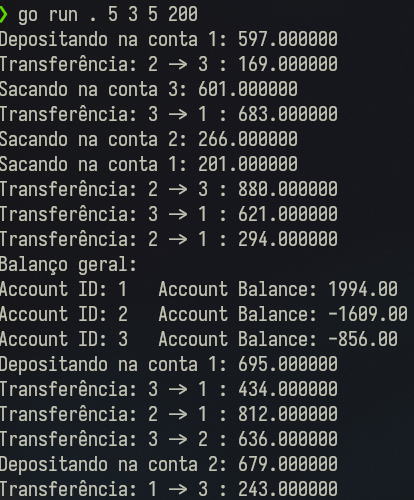
\includegraphics[scale=0.50]{2.png}
	\end{subfigure}
\end{figure}

\section*{Conclusões}
Ao variar os parâmetros do sistema, observou-se que o número de threads no pool influencia diretamente
a capacidade de processamento simultâneo do servidor. Um pool maior tende a reduzir o tempo de resposta
das requisições sob cargas mais altas, mas aumenta o uso de recursos e a complexidade do gerenciamento
de sincronização. Esses experimentos permitiram entender a importância de uma configuração equilibrada
para otimizar o desempenho do servidor multithreaded conforme os requisitos de cada cenário.
\end{document}
